\documentclass[11pt]{article}
\usepackage[utf8]{inputenc}
\usepackage[french]{babel}
\usepackage{graphicx}
\usepackage[T1]{fontenc}
%\usepackage{amss}
\usepackage{amsmath}
\usepackage{amsfonts}
\usepackage{amssymb}

\usepackage[left,modulo]{lineno}
\linenumbers

\newcommand\comment{}
\def\N{\mathbb N}
\def\R{\mathbb R}
\def\Q{\mathbb Q}
\def\Z{\mathbb Z}
\begin{document}
\title{EXAMEN I31 SESSION 2, 2015 - 2016}
\date{}\maketitle

Tous vos documents sont autorisés, mais pas la copie de votre voisin.
N’écrivez aucun programme. Ecrivez lisiblement. Répondez aux questions
dans l’ordre, en indiquant le numéro de chaque question.

\medskip
Lisez tout l'énoncé avant de commencer à répondre aux questions.

{
\section*{1. Euclide et Bézout (barême : 3 pts)}

En utilisant l'algorithme d'Euclide étendu, calculez le pgcd de 128 et 100 ainsi que les coefficients de Bezout $u$ et $v$, tels que~:
$$u\in \Z, v\in \Z, 128u + 100 v=\mbox{PGCD}(128, 100)$$
Complétez le tableau ci-dessous. Attention~! $u$ et $v$ sont des fonctions 
de $k$, le coefficient $v$  à la dernière ligne. 

\medskip
{\small
\begin{tabular}{|p{1.3cm}|p{1.3cm}|p{1.3cm}|p{1.3cm}|p{1.3cm}|p{1.3cm}|p{1.3cm}|}
\hline a & b & r=a\%b & q=a$\div$ b & pgcd(a,b) & u & v\\ 
\hline 
\hline  
128   &  100   &      &     &    &   &  \\
\hline  
&   &  &  &   &  &   \\
\hline 
 &   & & & &   &  \\
\hline 
 &   & & & &   &  \\
\hline  
 &   & & & &   &  \\
\hline
&  0  & --   & --   & 4 &  1 & k   \\
\hline
\end{tabular}
}
}

{
\section*{2. Equation de récurrence et complexité (barême : 2.5 pts)}
A. Pour le tri par fusion, quelle est l'équation récursive
donnant le temps  (ou  le nombre d'instructions élémentaires) $T(n)$ nécessaire pour trier $n$ éléments~? 


Vous prendrez $T(0)=1$ comme initialisation et $2n$ comme coût de la fusion des deux moitiés d'un tableau de $n$ éléments. 

\medskip
B. Quelle est la solution de cette équation~? Indication~: ce n'est pas $O( n^2)$.

\medskip
C. Quelle est la complexité des tris optimaux, en ne considérant que les tris effectuant des comparaisons ?

\medskip
D. Citez deux algorithmes qui trient des entiers sans les comparer.

\medskip
E. Quelle est la complexité du tri naïf~?
}
{
\section*{3. Sous mot commun le plus long (barême : 4 pts)}
Soit un mot $A$ et un mot $B$. 
Par exemple $A=6878568$ et $B=857686$. 
Les indices commencent à 1, par commodité~: $A_1=6, A_2=8$.
Les sous-mots les plus longs et communs à $A$ et à $B$ sont
8786, 8768, et 8568. Les lettres ne sont pas forcément consécutives, mais l'ordre des lettres dans les deux mots doit être préservé.

\medskip
Trouver le mot commun le plus long se ramène à calculer le chemin critique dans un graphe. En suivant les instructions ci-dessous, tous les arcs de votre graphe vont dans la même direction (de gauche à droite et en montant):

\begin{itemize}
\item tracez le graphe sur une grille ayant les chiffres de B sur les lignes et les chiffres de A sur les colonnes,
\item un sommet $S_{lc}$ est placé à l'intersection d'une ligne horizontale $l$ et d'une droite verticale $c$ chaque fois que  $A_c$ égale $B_l$,
\item   il y a un arc entre $S_{ij}$ et $S_{mn}$ ssi $i<m$ et $j<n$,
\item les arcs de transitivité sont facultatifs, 
\item par commodité, un sommet source $S_{00}$ et un sommet puits $S_{\infty\infty}$ sont ajoutés.
\end{itemize}

\medskip
A. Dessinez le graphe pour l'exemple $A=6878568$ et $B=857686$.
En supposant que tous les arcs ont une durée de 1, notez les dates au plus tôt
et au plus tard sur chaque sommet du graphe. Déduisez-en les chemins critiques.
Quels sont-ils~? 

\medskip
B. Dans cette question, l'ordre  entre les lettres n'a plus d'importance~:
le mot commun le plus long entre $A=1123$ et $B=2141$ est $112\equiv 121\equiv 211$, mais chaque lettre de $A$ ne peut être appariée 
qu'avec une seule des lettres identiques de  $B$. 
Décrivez {\bf en français} une méthode efficace pour résoudre ce problème (sans utiliser de graphe).

\medskip
C. Quand le graphe est sans cycle, trouver le chemin le plus long est possible en temps polynômial. Pour un graphe général (qui peut avoir des cycles), est-ce toujours vrai~? Le chemin doit être sans répétition de sommet.

\medskip
D. En A, nous avons utilisé de la programmation dynamique. Citez un autre problème soluble avec de la programmation dynamique.
}


{
\section*{4. Résoudre (barême : 3 pts)}
A. Résoudre $2^x= 3^k$. L'inconnue est $x$.

\medskip
B. Résoudre $2^k= \exp x$, où l'inconnue est $x$. Remarque~: $\exp x$ est aussi noté $e^x$, avec $e$ la base des logarithmes naturels.  

\medskip
C. Résoudre $a=\log x$. L'inconnue est $x$.
}

\section*{5. Suite (barême: 3.5 pts)}
On note $S_{a,b}$ une suite vérifiant~: $S_{a,b}(0)=a, S_{a,b}(1)=b$
et  la relation de récurrence~: $S_{a,b}(n)= 3 S_{a,b}(n-1) - 2 S_{a,b}(n-2)$ pour $n\ge 2$.

\medskip
Pour alléger, on écrit $s_0$ pour $S_{a,b}(0)$, $s_1$ pour $S_{a,b}(1)$
et, de façon générale, $s_i$ pour $S_{a,b}(i)$.

\medskip
A. Ecrivez  $s_n$ en fonction de  $s_{n-1}$ et  $s_{n-2}$, pour $n\ge 2$.

\medskip
B. Complétez le tableau suivant. 
$$
\begin{array}{|c|c|c|c|c|c|c|}
\hline
& s_0=a\; &  s_1=b\; & s_2\;  & s_3\;  & s_4\;  & s_5\;  \\
\hline 
S_{0,1} & 0 & 1 & & & &  \\
S_{1,0}  & 1 & 0 & & & &  \\
S_{1,1}  & 1 & 1 & & & & \\
S_{1,2}  & 1 & 2 & & & & \\
S_{2,1} & & & & & &\\
\hline 
\end{array}
$$

\medskip
C. Que remarquez-vous sur $S_{0,1}(n)$ et $S_{1,0}(n)$ ? que pouvez-dire du rapport de  $S_{a,b}(n)$  avec $S_{0,1}(n)$ et $S_{1,0}(n)$ ?

\medskip
D.
Complétez la matrice~:
$$
\left( \begin{array}{c}
s_2 \\
s_1 \end{array} \right) = \left( \begin{array}{cc}
~ & ~ \\
~ & ~ \end{array} \right) \left( \begin{array}{c}
s_1 \\
s_0 \end{array} \right)
$$

   
\medskip
E. Complétez la matrice et la puissance~:
$$
\left( \begin{array}{c}
s_n \\
s_{n-1} \end{array} \right) = \left( \begin{array}{cc}
~ & ~ \\
~ & ~ \end{array} \right) \left( \begin{array}{c}
s_1 \\
s_0 \end{array} \right)
$$

\iffalse
Rappel. Le déterminant de $$\left(\begin{array}{cc} A & B \\
C & D \end{array}\right)$$ est $AD-BC$.

\medskip
E. Le déterminant de $M-\lambda I_{2, 2}$, où $M$ est la matrice précédente, et $I_{2, 2}$ la matrice identité, est un polynôme en la variable $\lambda$. Que vaut-il~?  Quelles sont les deux racines de ce polynôme en $\lambda$~? Appelons les $\lambda_1$ pour la plus petite, et $\lambda_2$ pour la plus grande.


\medskip
F. En fait, $S_{a,b}(n) = \alpha_1 \lambda_1^n + \alpha_2\lambda_2^n$.
Quelles sont les valeurs de $\alpha_1$ et $\alpha_2$ 
(en fonction de $a$ et $b$)  qui sont telles que
$S_{a,b}(0)=a$, et $S_{a,b}(1)=b$~?

\medskip
G. Toutes les suites $S_{a,b}$ sont périodiques modulo $m$, un nombre entier non nul.
Quelle est la longueur maximale de la période, en fonction de $m$~? Expliquez pourquoi~?

\fi

\section*{6. Puissance de matrice (barême: 4 pts)}

A. Quel est le nombre minimal de produits de matrices à effectuer pour calculer $M^k$, où $M$ est une matrice donnée, et $k\in \N$ est un entier donné~?
Rappelez les formules récursives de la puissance rapide d'une matrice. Une telle matrice peut-elle être non carrée~?

\medskip
B. Travaillons maintenant sur une matrice diagonale, $D$, et
notons la diag$(d_1, d_2, \ldots d_n)$. Ainsi la matrice identité est 
diag$(1, \ldots 1)$. Que vaut $D^k$, avec $k\in \N$, et $D=\mbox{diag}(d_1, d_2, \ldots d_n)$~?
Quel est l'intérêt, relativement à la question précédente~?

\medskip
C. Soient trois matrices $M, D, V$ telles que~: 

\begin{itemize}

\item $MV=VD$,
\item la matrice $V$ est inversible (sa matrice inverse est notée  $V^{-1}$ et le produit $V V^{-1}$ est la matrice identité),
\item la matrice $D$ est diagonale.

\end{itemize}

\medskip
\emph{Par exemple les trois matrices décrites ci-dessous sont 
conformes à cette définition.}
$$M=\left( \begin{array}{cc} 3 & -2\\
1 & 0 
\end{array}\right), \quad D=\left( \begin{array}{cc} 1 & 0 \\
0 & 2 \end{array}\right), \quad V=\left( \begin{array}{cc} 1 & 2 \\
1  & 1 \end{array}\right), \quad V^{-1}=\left( \begin{array}{cc} -1 & 2 \\
1  & -1 \end{array}\right) $$
 


Déduisez-en une formule explicite pour $M^k$, avec $k\in \Z$,
où les seules puissances de matrices sont des puissances de $D$.
Vous devez travailler dans le cas général: ne remplacez pas $D, V, V^{-1}$ par leur valeur.

%%\comment{D. Déduisez-en une formule explicite pour $M^k$, avec $k\in \R$~: vous avez le droit d'utiliser les fonctions $\log$ et $\exp$, mais vous n'avez pas le droit d'utiliser la fonction appelée pow en C (elle calcule $u^v$, avec $u$ et $v$ deux nombres de type double).  }

\medskip
D. La matrice $M$ a déjà été rencontrée. Donnez une formule matricielle explicite pour calculer $S_{a,b}(n)$, où les seules puissances de matrices sont des puissances de $D$.
Ne remplacez pas $D, V, V^{-1}$ par leur valeur.






\end{document}
\newpage
{
\section{Euclide et Bézout}

En utilisant l'algorithme d'Euclide étendu, calculez le pgcd de 128 et 100 ainsi que les coefficients de Bezout $u$ et $v$, tels que~:
$$u\in \Z, v\in \Z, 128u + 100 v=\mbox{PGCD}(128, 100)$$
Complétez le tableau ci-dessous. Attention~! $u$ et $v$ sont des fonctions
de $k$, le coefficient $v$  à la dernière ligne.

Solution.

\begin{tabular}{|p{1.5cm}|p{1.5cm}|p{1.5cm}|p{1.5cm}|p{1.5cm}|p{1.5cm}|p{1.5cm}|}
%\hline a & b & r=a\%b & q=$\lfloor$ a/b$\rfloor$ & pgcd(a,b) & u & v\\ 
\hline a & b & r=a\%b & q=a$\div$ b & pgcd(a,b) & u & v\\ 
\hline 
\hline  
128   &  100   & 28    & 1    & 4   & 25k-7  & -32k+9 \\
\hline  
100 & 28   & 16  & 3 & 4  & -7k+2 &  25k-7 \\
\hline 
28 & 16   & 12  & 1 & 4  & 4k-1  & -7k+2 \\
\hline 
16 &  12  &  4 &  1  & 4 &  -3k+1 & 4k-1  \\
\hline  
12 &  4  & 0   & 3   & 4  &  k & 3k+1  \\
\hline
4 &  0  & --   & --   & 4  &  1 & k   \\
\hline
\end{tabular}
}

{
\section{Equation de récurrence et complexité}
A. Pour le tri par fusion, quelle est l'équation récursive
donnant le temps $T(n)$ (ou  le nombre d'instructions élémentaires) nécessaire pour trier $n$ éléments~? Vous prendrez $T(0)=1$.


Réponse. $T(n)= 2 T(n/2) + n$. La solution est $T(n)= O(n \log n)$.

B. Quelle est la solution de cette équation~? Indication~: ce n'est pas $O( n^2)$.

Réponse. La solution est $T(n)= O(n \log n)$.

C. Quelle est la complexité des tris optimaux, en ne considérant que les tris effectuant des comparaisons ?

Réponse. $(n \log n)$.

D. Citez deux algorithmes qui trient des entiers sans les comparer.

Tri par tiroir ("bucket sort"), et tri par base ("radix sort").

E. Quel est la complexité du tri naïf~?

Réponse. $O(n^2)$.

}
\section{Sous mot commun le plus long}
A. A un renommage près, le problème est le même que dans


\verb&http://ufrsciencestech.u-bourgogne.fr/master1/mi1-tc5/EN_VRAC/PLSSC/pluslongcommun.pdf&

Une des solutions a été oubliée Fig. 1.

B. Supposons que $A$ et $B$ sont deux ensembles -- l'ordre entre les lettres n'a pas d'importance. Cependant, chaque lettre de $A$ ne peut être appariée
qu'avec une seule lettre (identique) dans $B$.
Décrivez {\bf en français} une méthode efficace pour résoudre ce problème.

Réponse. Pour chaque lettre de $A$, compter combien de fois elle apparaît dans
$A$ et dans $B$ (en utilisant une table de hachage par exemple).
Si une lettre apparaît $a$ fois dans $A$ et $b$ fois dans $B$,
alors elle apparaît $\min(a, b)$ dans le multi-ensemble intersection de $A$ et de $B$.

C. Quand le graphe est sans cycle, trouver le chemin le plus long est possible en temps polynômial. Pour un graphe général (qui peut avoir des cycles), est-ce toujours vrai~? Le chemin doit être sans répétition de sommet.

Réponse. Non, c'est un problème difficile, qui généralise le problème du chemin hamiltonien.

D. En A, nous avons utilisé de la programmation dynamique. Citez un autre problème soluble avec de la programmation dynamique.

Réponse.
Pour le sac à dos, pour le parenthésage optimal de produits de matrices, pour la séquence croissante la plus longue, pour la distance d'édition entre deux mots,
pour le calcul des chemins critiques dans les graphes, et beaucoup d'autres.
 
{
\section{Résoudre}
A. Résoudre $2^x= 3^k$. L'inconnue est $x$.

Solution~:
$$2^x= 3^k\Rightarrow x \log 2 = k \log 3 \Rightarrow x = k \log 3 / \log 2$$

B. Résoudre $2^k= \exp x$, où l'inconnue est $x$. Remarque~: $\exp x$ est aussi noté $e^x$, avec $e$ la base des logarithmes naturels.

Solution~:
$$2^k= \exp x \Rightarrow k \log 2 = \log \exp x = x $$

C. Résoudre $a=\log x$. L'inconnue est $x$.


}

\section{Suite}
On note $S_{a,b}$ une suite vérifiant~: $S_{a,b}(0)=a, S_{a,b}(1)=b$
et  la relation de récurrence~: $S_{a,b}(n)= 3 S_{a,b}(n-1) - 2 S_{a,b}(n-2)$ pour $n\ge 2$.


A. Complétez le tableau suivant.
$$
\begin{array}{|c|c|c|c|c|c|c|}
\hline
& s_0\; &  s_1\; & s_2\;  & s_3\;  & s_4\;  & s_5\;  \\
\hline
S_{0,1} & 0 & 1 & 3 & 7  & 15 & 31 \\
S_{1,0} & 1 & 0 & -2 & -6 & -14 & -30  \\
S_{1,1} & 1 & 1 & 1 & 1 & 1 & 1 \\
S_{1,2} & 1 & 2 & 4 & 8 & 16 & 32 \\
S_{2,1} & 2 & 1 & -1 & -5 & -13 & -29\\
\hline
\end{array}
$$

B. Que remarquez-vous entre  d'une part~:
$S_{0,1}(n)$ et $S_{1,0}(n)$,  et d'autre part~: $S_{a,b}(n)$ ?

Réponse~: $$S_{a,b}(n)= a S_{1,0}(n) + b S_{0,1}(n)$$

C.
Complétez la matrice~:
$$
\left( \begin{array}{c}
s_2 \\
s_1 \end{array} \right) = \left( \begin{array}{cc}
3 & -2 \\
1 & 0 \end{array} \right) \left( \begin{array}{c}
s_1 \\
s_0 \end{array} \right)
$$

D. Complétez la matrice et la puissance~:
$$
\left( \begin{array}{c}
s_n \\
s_{n-1} \end{array} \right) = \left( \begin{array}{cc}
3 & -2 \\
1 & 0 \end{array} \right)^{n-1} \left( \begin{array}{c}
s_1 \\
s_0 \end{array} \right)
$$

E. Que vaut le déterminant de $M-\lambda I_{2, 2}$, où $M$ est la matrice précédente, et $I_{2, 2}$ la matrice identité~?  Quelles sont les deux racines de ce polynôme~?


Réponse~: $\lambda^2-3\lambda+2=(\lambda-1)(\lambda-2)$. Les deux racines sont 1 et 2.

F. Toutes ces suites $S_{a,b}$ sont périodiques modulo $m$, un nombre entier non nul.
Quelle est la longueur maximale de la période, en fonction de $m$~? Pourquoi~?

Réponse~: $m^2$. La suite est complètement fixée par deux termes consécutifs.
Appelons couple deux termes consécutifs. Par exemple, dans 10, 20, 30, 40,
les couples sont~: (10, 20), (20, 30), (30, 40)...
Donc la suite est complètement déterminée par le premier couple.
Mais il y a au plus $m^2$ couples distincts, modulo $m$.
Donc la période ne peut pas être plus longue que $m^2$ couples, donc
$m^2$ éléments (prendre le premier entier de chaque couple).

\section{Puissance de matrice}

A. Quel est l'ordre de grandeur du nombre minimal de produits de matrices pour calculer $M^k$, où $M$ est une matrice donnée, et $k\in \N$ est un entier donné~?
Rappelez les formules récursives. La matrice peut-elle être non carrée~?

Réponse. $O(\log k)$ produits matriciels sont nécessaires.
$M^0=I$, où $I$ est la matrice identité. 
Cas des puissances paires~: $M^{2k} = (M^2)^k$.
Cas des puissances impaires~:  $M^{2k+1} = M (M^{2k})$, ou bien
$M^{2k+1} = M (M^2)^{k}$. Donc chaque appel récursif divide la puissance par 2.
Au bout de $O(\log k)$ appels récursifs, on termine sur $M^0$.
La matrice doit être carrée~: dans un produit, le nombre de colonnes de la première matrice doit être égal au nombre de lignes de la seconde. Donc si les deux matrices sont identiques, le nombre de ligne doit égaler le nombre de colonnes.



B. Supposons $M$ diagonale. D'ailleurs appelons la $D$, et
notons la diag$(d_1, d_2, \ldots d_n)$. Ainsi la matrice identité est
diag$(1, \ldots 1)$. Que vaut $D^k$, avec $k\in \N$, et $D=\mbox{diag}(d_1, d_2, \ldots d_n)$~?

Réponse. $$D^k=\mbox{diag}(d_1^k, d_2^k, \ldots d_n^k)$$
L'intérêt est que cette formule ne nécessite aucun produit matriciel (un produit de matrice carrée de taille $n$ par $n$ est en $O(n^3)$, avec la méthode naïve).
 
Soient  les trois matrices $M, D, V$~:
$$M=\left( \begin{array}{cc} 3 & -2\\
1 & 0
\end{array}\right), \quad D=\left( \begin{array}{cc} 1 & 0 \\
0 & 2 \end{array}\right), \quad V=\left( \begin{array}{cc} 1 & 2 \\
1  & 1 \end{array}\right), \quad V^{-1}=\left( \begin{array}{cc} -1 & 2 \\
1  & -1 \end{array}\right) $$
Ces matrices sont telles que $MV=VD$, la matrice $V$ est inversible,
et $D$ est diagonale.

C. Déduisez-en une formule explicite pour $M^k$, avec $k\in \Z$.

Réponse~: $M^k= (VDV^{-1})^k = (VDV^{-1})(VDV^{-1})\ldots = VD^kV^{-1}$.
$D$ est une matrice diagonale, et son vecteur diagonal est $(1, 2)$. Donc $D^k$ est une matrice diagonale, et son vecteur diagonal est $(1, 2^k)$.

D. Déduisez-en une formule explicite pour $M^k$, avec $k\in \R$~: vous avez le droit d'utiliser les fonctions $\log$ et $\exp$.

Réponse~: idem. $M^x=VD^xV^{-1}$. Ici $D^x$ est une matrice diagonale, dont le
vecteur diagonal est $(1, 2^x)$. On a vu que $2^x =\exp( x \log 2)$.

E. Donnez une formule matricielle (avec un nombre constant de produits de matrices non diagonales)  pour calculer $S_{a,b}(n)$.

Réponse.  La première ligne est suffisante~:
\begin{eqnarray*}
\left( \begin{array}{c}
s_n \\
s_{n-1} \end{array} \right) & = & M ^{n-1} \left( \begin{array}{c}
s_1 \\
s_0 \end{array} \right) = V D^{n-1} V^{-1} \left( \begin{array}{c}
s_1 \\
s_0 \end{array} \right) \\
&=&  
V\left( \begin{array}{cc}
1 & 0 \\
0 & 2 ^{n-1}\end{array} \right) V^{-1}  \left( \begin{array}{c}
s_1 \\
s_0 \end{array} \right)  \\
&=&
V\left( \begin{array}{cc}
1 & 0 \\
0 & \exp( (n-1)\log 2 \end{array} \right) V^{-1}  \left( \begin{array}{c}
s_1 \\
s_0 \end{array} \right)
\end{eqnarray*}

F. En fait, $S_{a,b}(n)$ vaut $\alpha 1^n + \beta 2^n$. Exprimez $\alpha$ et 
$\beta$ en fonction de $a$ et $b$.

Réponse. $ S_{a,b}(0)= \alpha + \beta=a, \quad S_{a,b}(1)=  \alpha + 2 \beta= b$. Donc
$\alpha=2a-b $ et $\beta=b-a$. Donc 
$$ S_{a,b}(n) = 2a - b + (b-a)^n$$



\end{document}





\section{Quizz}

\begin{enumerate}
\item Citez deux problèmes indécidables en informatique.

\emph{La terminaison d’un algorithme (ou d’une machine de Turing), l’égalité de deux nombres réels (ou complexes), l’égalité de deux fonctions (par exemple de N dans N). }



\item  Quand dit-on qu'un problème est difficile en informatique.

{\it Quand aucun algorithme en temps polynomial permettant de résoudre ce problème n’est connu\footnote{Ce qui ne prouve pas qu'il n'en existe pas...}.

Quelques réponses fausses~: 

- quand il existe un algorithme en temps exponentiel. Or il existe un algorithme  en temps exponentiel pour le tri, tel que générer toutes les permutations possibles. 

- quand il n'existe qu'un ou des  algorithmes en temps non polynomial. Le problème avec cette réponse est~: pour certains problèmes, il n'y a pas d'algorithme
connu qui marche en temps polynomial, mais cela ne prouve pas qu'il n'en existe pas. Ainsi, personne ne sait prouver l'inexistence d'algorithme en temps polynomial pour résoudre les problèmes de la classe NP. 
}

\item  Citez deux problèmes solubles en informatique, mais difficiles.


\emph{Résoudre un problème SAT (où un solveur SAT est un programme qui décide automatiquement si une formule de logique
propositionnelle est satisfaisable). Trouver un chemin ou un circuit hamiltonie
n (passant par tous les sommets dans un graphe). Trouver une clique
ou un stable de taille maximale ou de taille fixée. Plus généralement, résoudre un problème de la classe NP. Factoriser un très grand entier est aussi un problème difficile, car aucun algorithme en temps polynomial n'est connu aujourd'hui. De même pour le problème du logarithme discret: résoudre $a^x=b \mod p$ où $p$ est un entier premier.}





\item Donnez deux algorithmes efficaces pour trier des nombres en utilisant
des comparaisons. Indiquez la complexité (en nombre de comparaisons)
de ces deux algorithmes. 
\begin{itemize}
\item  \emph{tri par fusion (mergesort, $O(n*log(n)$)}
\item  \emph{tri par tas (heapsort, $O(n*log(n)$)}
 \item  \emph{tri rapide (quicksort, en moyenne complexité en $O(n*log(n)$).}
\end{itemize}

\item   Donnez le nom de trois algorithmes calculant les plus courts chemins dans un graphe.

\emph{Dijkstra, Floyd, Ford (ou Ford-Bellman), Dantzig, Warshall, pseudo produit matriciel: $(AB)_{l,c}= min_k (A_{lk} + B_{kc})$.}

\end{enumerate}

\section{Ordonnancement}

\begin{center}
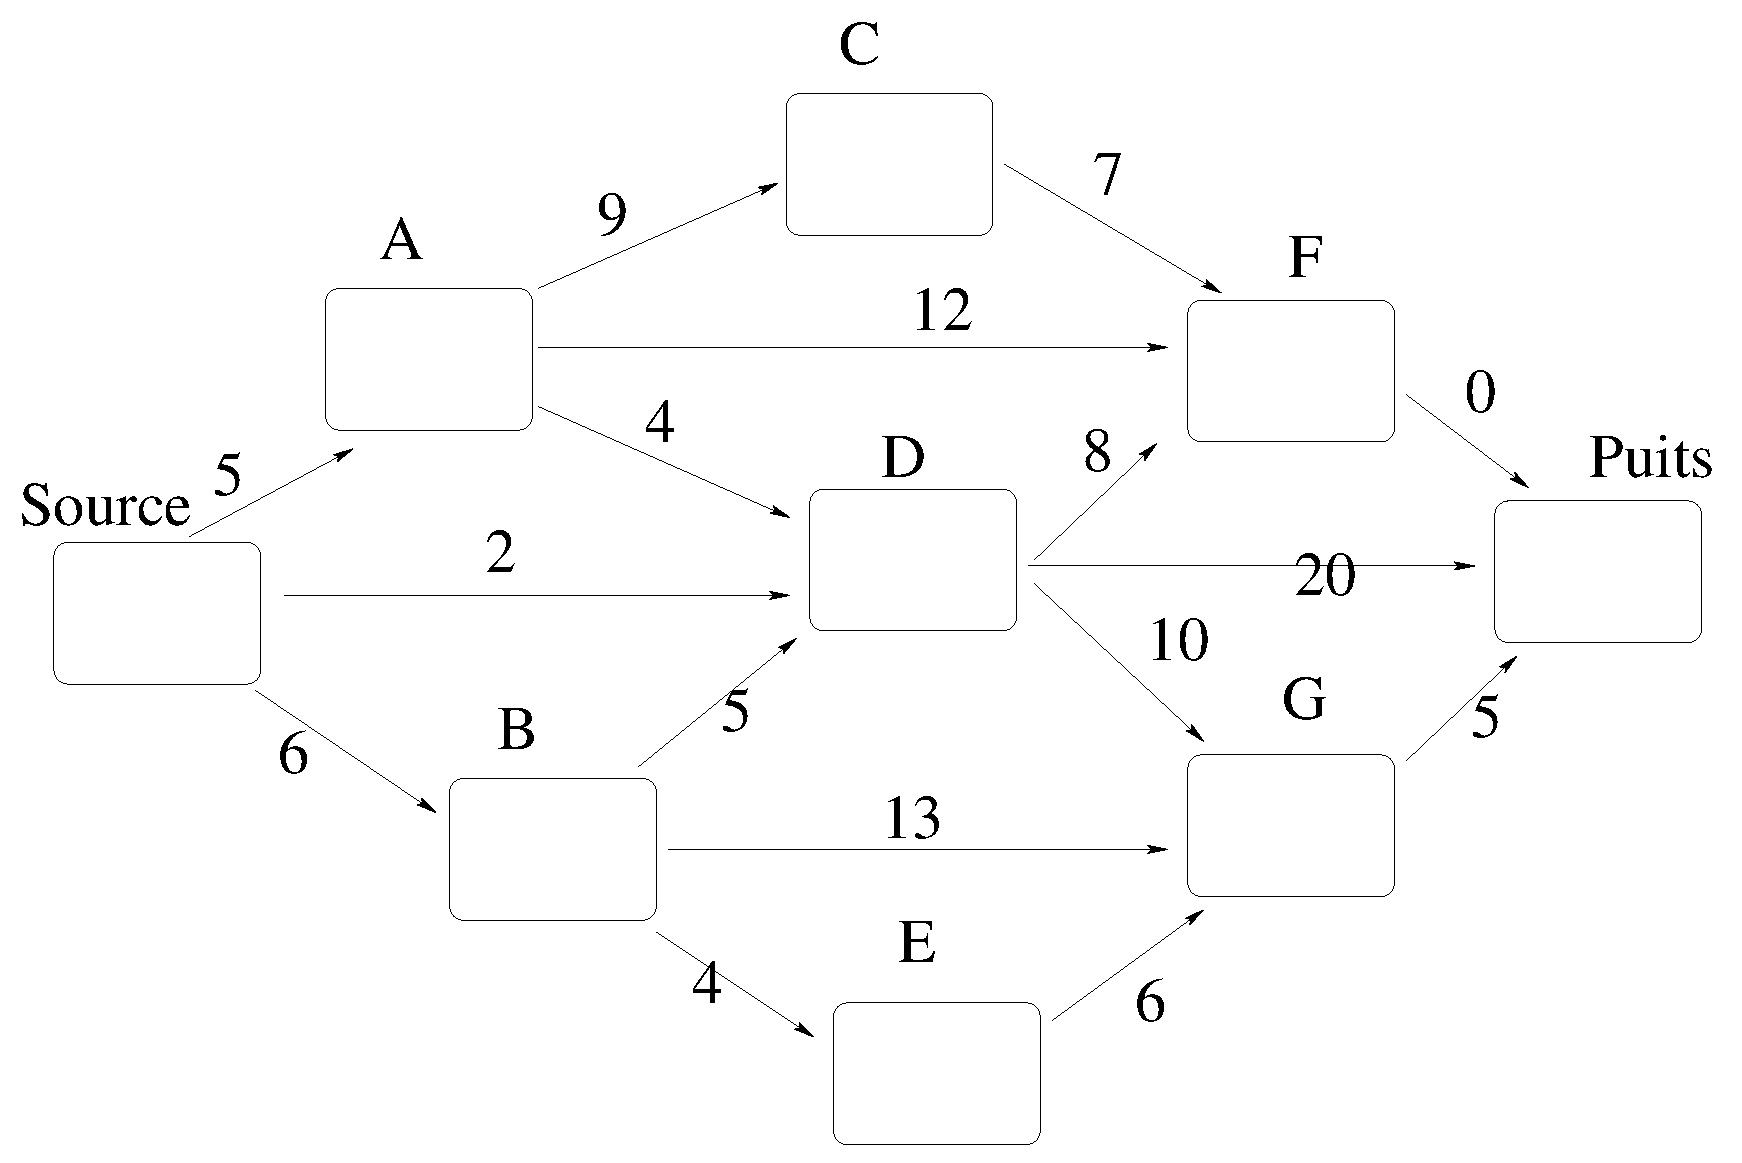
\includegraphics[width=0.95\linewidth]{critique.eps}
\end{center}


Etant donnée la description des tâches donnée ci-dessus: 

\begin{enumerate}

\item 
En calculant de SOURCE vers PUIT, complétez les dates au plus tôt (comme par exemple 0- et 5-).


Puis en calculant de  PUIT vers SOURCE, complétez les dates au plus tard (comme par exemple -0 et -7).

Soulignez le chemin critique.

\begin{center}
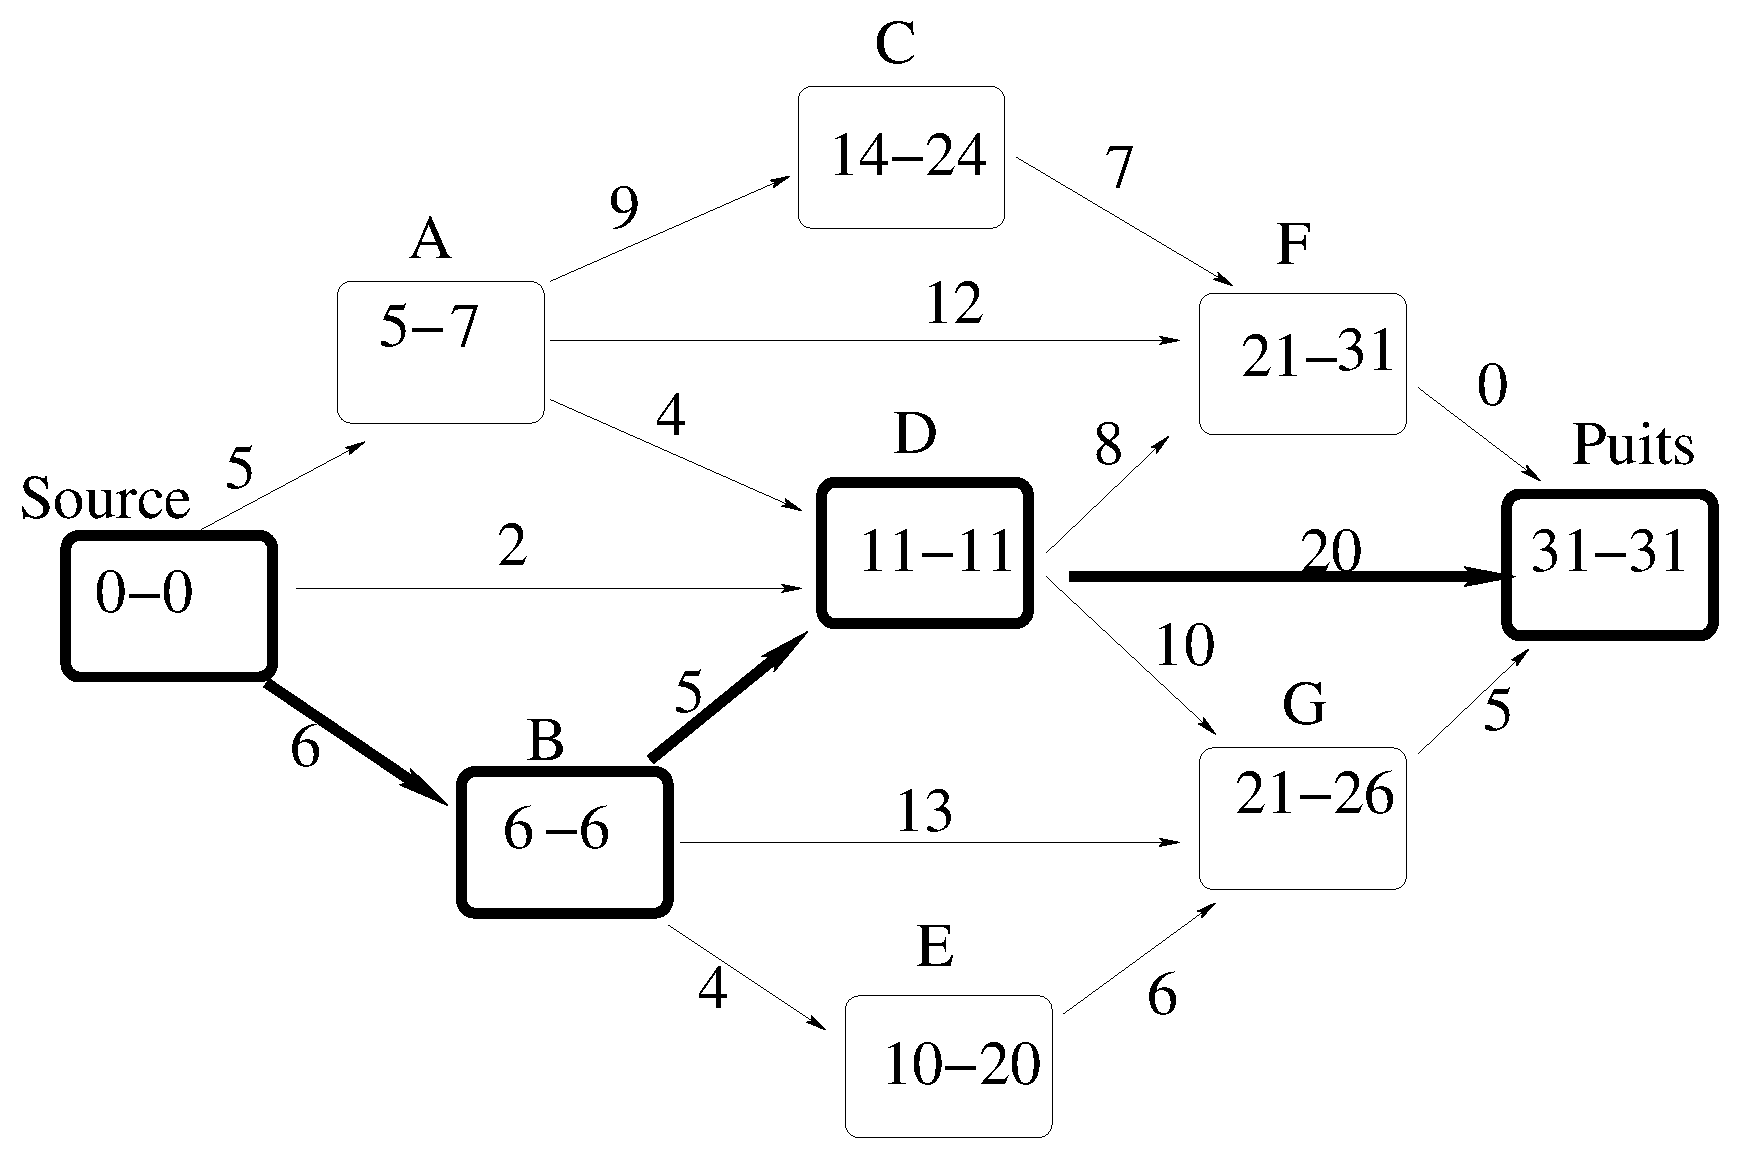
\includegraphics[width=0.95\linewidth]{critique_solution.eps}
\end{center}

%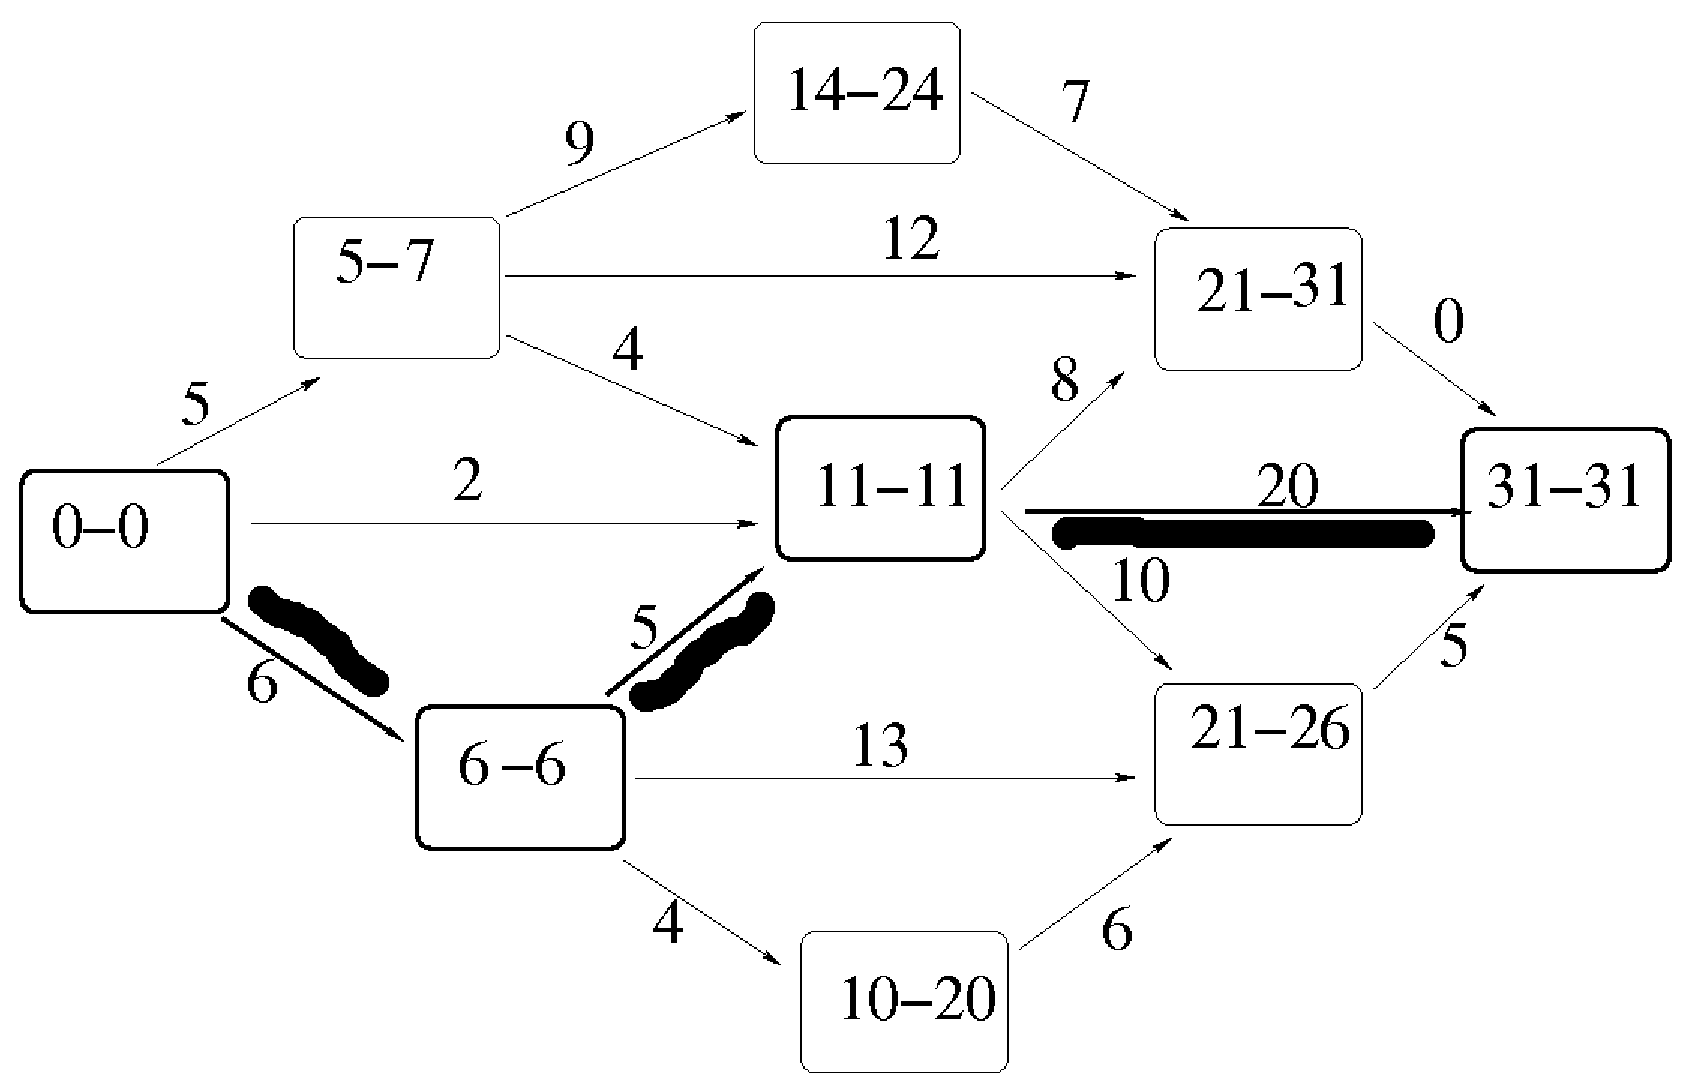
\includegraphics[width=0.95\linewidth]{critique_solutionCHEMIN.eps}



\item Que faire si le graphe a plusieurs sommets sources (ou puits) ?

\emph{Si un graphe a plusieurs sources, on peut ajouter une source virtuelle
$\Omega$  reliée à toutes les sources $s$  par un arc $\Omega\rightarrow s$  de durée nulle.}

 \emph{De même pour un graphe ayant plusieurs puits.
Chaque  puits $p$ est relié à un sommet terminal $P$  par un arc
$s\rightarrow P$ de durée nulle. 
}

\item  Vous pouvez supposer que le graphe est acyclique, qu'il a un seul sommet source, un seul sommet puits, et que les durées sur les arcs sont non négatives.
Donnez la définition, en français, de la date au plus
tôt. Prévoyez bien tous les cas : sommet avec ou sans arc entrant ou
sortant.

%\emph
{\it
$s$ est la source  $\Rightarrow \mbox{Tôt}(s) = 0$

Sinon~:
$$\mbox{Tôt}(s)= \max_{r:\; r\rightarrow s} \mbox{Tôt}(r)+ C(r\rightarrow s)$$
c'est à dire le maximum, pour tous les
sommets $r$ tels qu'il existe un arc $r\rightarrow s$,  des 
$\mbox{Tôt}(r)+\mbox{Durée}(r\rightarrow s)$.

Remarque~: la date au plus tôt de $s$ est la longueur du chemin le plus {\bf long} de la source jusqu'à $s$, et non pas le chemin le plus court. Ici, ce problème est facile car le graphe est acyclique~; rappelons que calculer le chemin (acyclique) le plus long dans un graphe avec cycle  est difficile~: le chemin hamiltonien est un cas particulier de ce problème où tous les coûts sont égaux (à 1 par exemple).
}

\item   Donnez la définition, en français, de la date au plus tard. Prévoyez bien tous les cas.

%\emph
{\it
$s$ est le puits  $\Rightarrow \mbox{Tard(s)= Tôt}(s)$.

Sinon~:
$$\mbox{Tard}(s)=\min_{t:\; s\rightarrow t} \mbox{Tard}(t) - \mbox{Durée}(s\rightarrow t)$$
}

\item   Quand un sommet est-il critique~?

\emph{Lorsque ses dates au plus tôt et au plus tard sont identiques.}
\end{enumerate}

\section{Dessinez le graphe d'un jeu de Nim}
Deux joueurs jouent à tour de rôle (Albert commence, Bertrand joue en second). Sur la table, il y a trois tas de pions~:
deux tas de 2 pions, et un tas de 1.

\smallskip
Chacun des joueurs choisit un tas (non vide) et  un seul,
et en retire un nombre entier  non nul  de pions~; il peut retirer  tous les pions du tas s'il le souhaite.

\smallskip
Le premier joueur qui ne peut plus retirer de pions
a perdu, ou, le premier joueur qui enlève tous les pions restant dans le dernier tas a gagné. 

\medskip
Vous utiliserez une représentation des états par niveaux: le niveau $n$ contient les états où la somme des nombres de pions vaut $n$ ($0 \le n \le 6 $). Un seul des états équivalents est représenté ($(2, 1, 1)=(1, 2, 1)=(1, 1, 2)$) et les $0$ inutiles sont éliminés.

Par exemple le niveau 2 contient
les états $(2)$ et $(1, 1)$. 

\medskip
Un sommet est gagnant si et seulement si le joueur qui y arrive peut toujours gagner, quels que soient les coups joués par l'adversaire.
Un sommet est perdant si et seulement si il n'est pas gagnant.


 \begin{enumerate}
\item  Le schéma fourni ne contient que les niveaux 0, 1, 2. Ajoutez les 4 états
manquants.

\emph{Voir Figure ci-dessous.}

\item  Sur le graphe, dessinez les arcs de tous les coups possibles ; il y a 16
arcs en tout ; chaque état est représenté par un sommet ; un arc va d’un
sommet $s$ à un sommet $t$ quand il est possible de passer en un coup de
$s$ à $t$.


\emph{Voir Figure ci-dessous.}


\item Marquez chaque sommet $G$ s’il est gagnant et $P$ s’il est perdant. Epaississez le contour des sommets gagnants.


\emph{Voir Figure ci-dessous.}


\item  Quel joueur, Albert ou Bertrand, est sûr de gagner, s'il joue intelligemment, bien sûr~?

\emph{Albert est sûr de gagner s'il enlève le pion isolé. }

\item Décrivez l'algorithme que vous avez utilisé pour marquer les sommets  $G$ ou $P$.

\emph{La position finale est gagnante. Il faut "remonter" vers la position initiale avec :}
\begin{itemize}
\item \emph{une position ayant au moins un arc  vers une position gagnante est perdante}
\item \emph{dit autrement, une position dont tous les arcs sortants mènent à une position perdante est gagnante}
\end{itemize}

\item  Dans un graphe orienté acyclique (c'est le cas ici), un noyau $N$ est 
un sous-ensemble de sommets du graphe tel que~: si $s$ est dans $N$, tous ses voisins sont hors de $N$~; si $s$ est hors de $N$, il existe au moins un arc vers un sommet $t$ qui se trouve dans $N$. 

Quel est le lien avec le problème précédent~? 

\emph{Les positions gagnantes forment un noyau.}

\end{enumerate}

\bigskip

\begin{center}
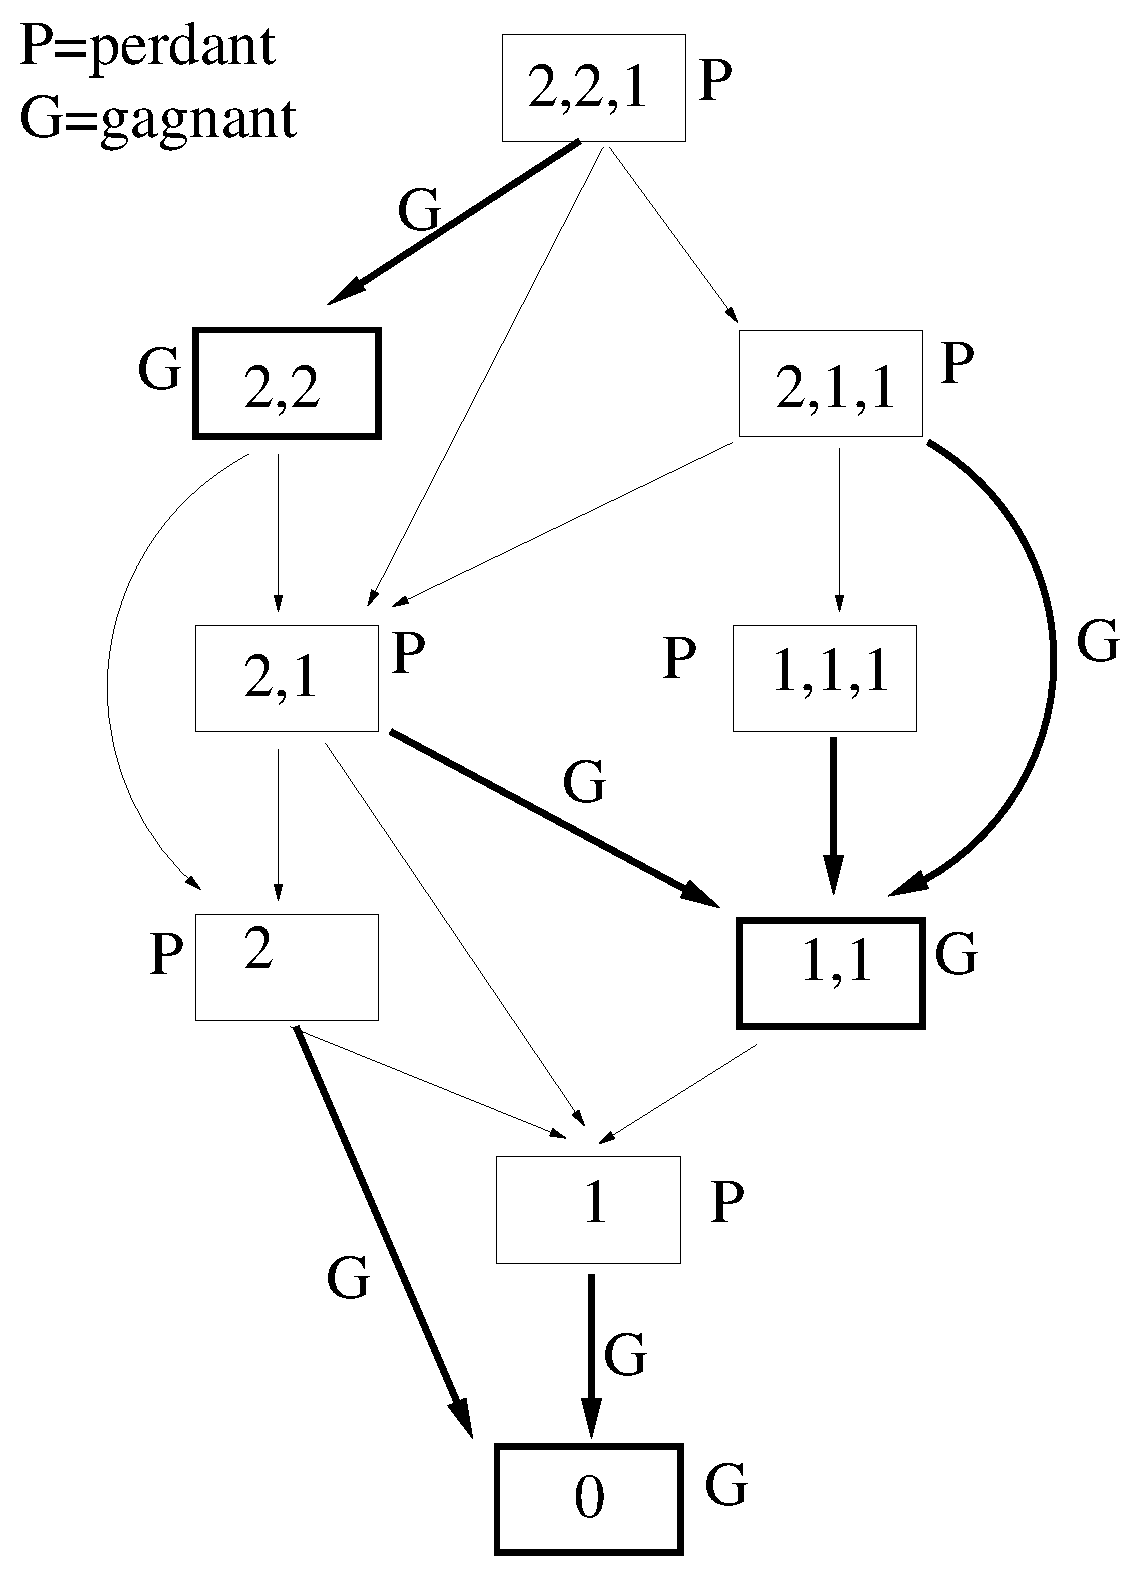
\includegraphics[width=0.75\linewidth]{nim.eps}
\end{center}
Remarque sur le dessin du graphe~: il est bien précisé dans l'énoncé de dessiner niveau par niveau, et qu'un seul sommet doit être dessiné quand plusieurs états sont équivalents~: $(2,1,1)=(1,2,1)=(1,1,2)$, etc.


\end{document}
{
\section{La méthode de Karatsuba}

La méthode scolaire pour additionner deux grands entiers est optimale, car proportionnel au nombre de chiffres du plus grand des deux nombres.
La  méthode scolaire pour multiplier deux nombres de deux chiffres en base $B$
(par exemple $B=10000$, dix mille) ne l'est pas. Karatsuba a découvert une méthorécursive meilleure.
Pour calculer
$(a + b G) (a' + b' G)=aa' + (ba'+a'b) G + bb' G^2$ où $G$ est une puissance entière de la base $B$, Karatsuba propose de calculer récursivement~:
$U=aa'$, $V=bb'$, $W=(a+b)(a'+b')$ et 
remarque que $ba'+a'b=W-U-V$.
Ainsi le produit de deux nombres de $n$ chiffres en base $B$ requiert
trois produits  de deux nombres de $n/2$ chiffres en base $B$ (au lieu de quatre pour la méthode naïve). Les  trois additions $a+b$, $a'+b'$ et $U+V$
 et la soustraction $W-(U+V)$ de nombres de $n/2$ (ou $1+n/2$ chiffres n'ont pas d'importance. 

La formule récursive pour  $T(n)$, l'ordre de grandeur du nombre d'instructions nécessaire pour calculer le produit de deux nombres de $n$ chiffres en base $B$ par la méthode naïve, est~: $T(0)=1, T(n)=4T(n/2)+n$. La solution est $T(n)=O(n^2)$~; cela se voit plus facilement si on considère $T(n)=4T(n/2)$.

Donnez la formule récursive pour  $T(n)$, l'ordre de grandeur du nombre d'instructions nécessaire pour calculer le produit de deux nombres de $n$ chiffres en base $B$ par la méthode de Karatsuba.

Résoudre l'équation de récurrence $T(n)=3T(n/2)$.
}
